\pagebreak
\subsection{Electrical Design}

\subsubsection{Block Diagrams}
\begin{centering}
The electronics design can be seen in Figure \ref{fig:electronics-block-diagram} and the interfaces this requires can be seen in Figure \ref{fig:eee-interface-diagram}. There will be four distinct areas, the Electronics box, the valve centre, the pump box and the CAC system. All connections to the outside of the box are located in the electronics box. These are the voltage regulators for the external power source and the Ethernet shield with an SD data storage which will connect to the Telemetry, Tracking, and Command (TT\&C). Additionally three pressure sensors, one heater and one temperature sensor will be placed in this area. The CAC system area will contain three temperature sensors to monitor the ambient temperature and one electronic valve to be closed before landing. In the AAC system area there will be nine valves, one airflow sensor, three pressure sensor, four temperature and one humidity sensor and a heater. In the pump box there will be the miniature diaphragm air pump, one temperature sensor and one heater. 
\end{centering}
\bigskip

\begin{figure}[H]
    \begin{align*}
        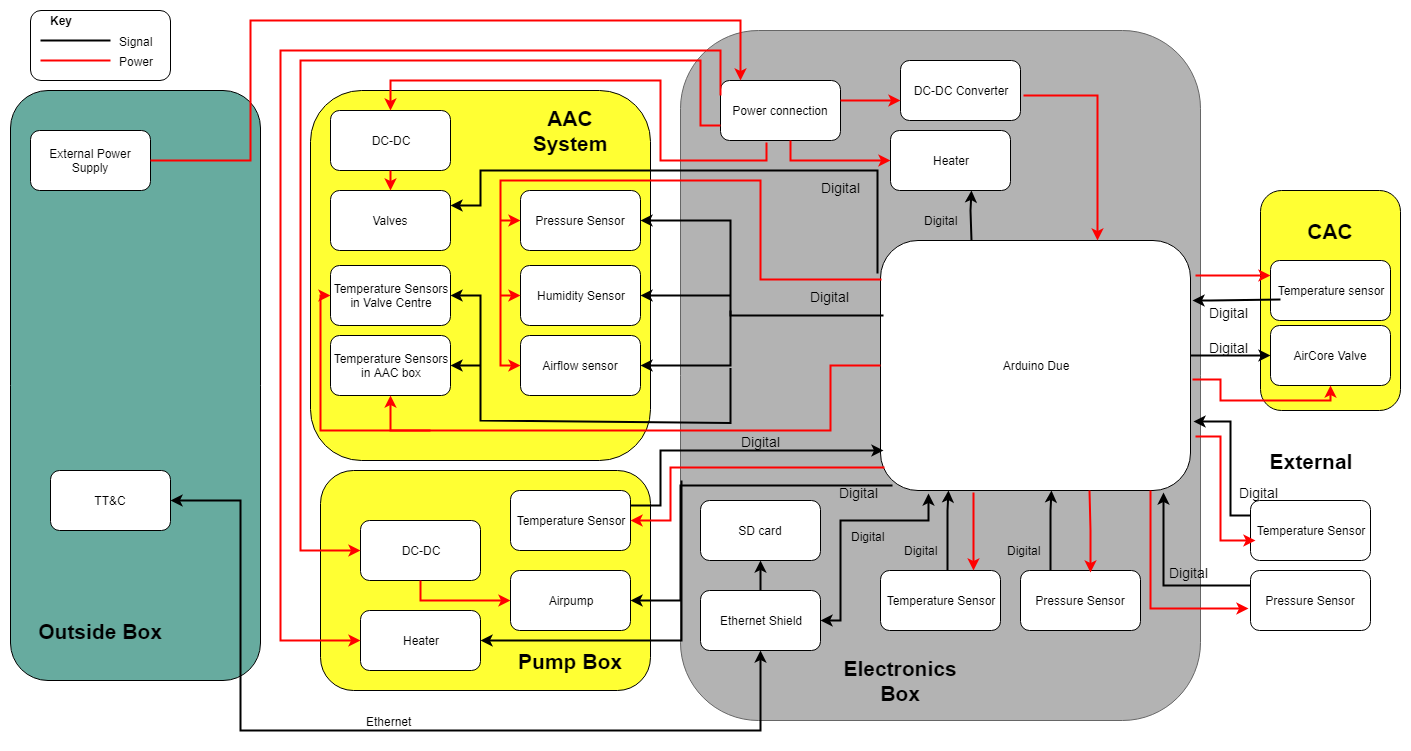
\includegraphics[width=16cm]{4-experiment-design/img/block-diagram-four-sections.png}
    \end{align*}
    \caption{Block Diagram for all Electronic Components Showing the Signal and Power Connections}\label{fig:electronics-block-diagram}
\end{figure}


\begin{figure}[H]
    \begin{align*}
        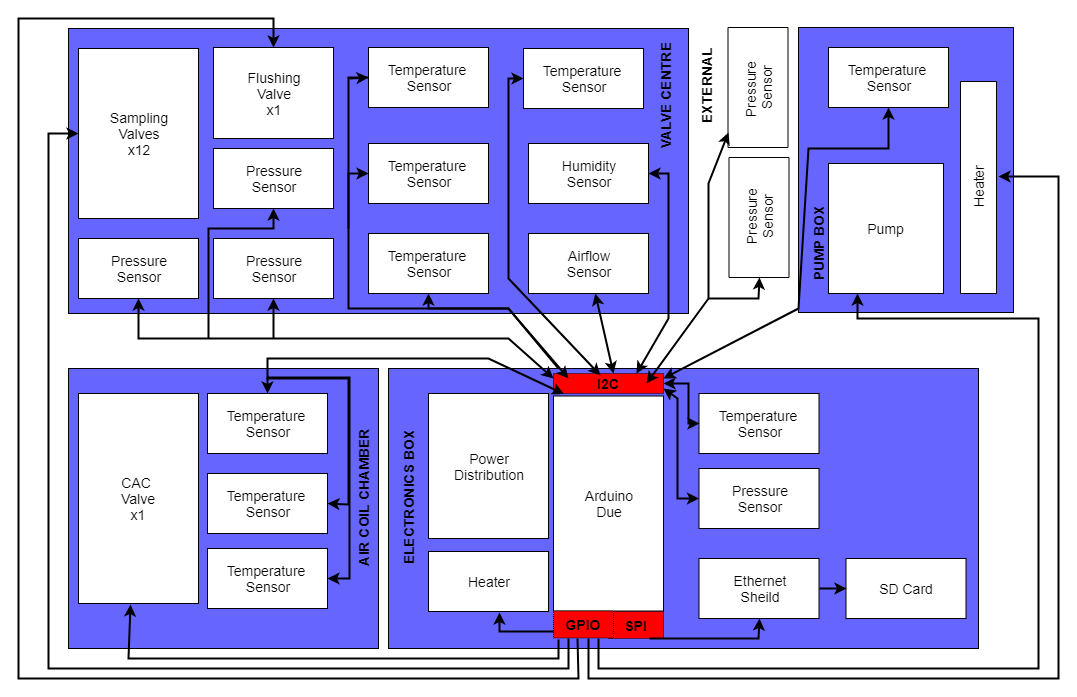
\includegraphics[width=16cm]{4-experiment-design/img/interface-diagram-v2.png}
    \end{align*}
    \caption{Block Diagram Showing the Interfaces Between All Electrical Components.}\label{fig:eee-interface-diagram}
\end{figure}

\begin{centering}
Three DC-DC converters will be used to step down the voltage from the 28.8V provided by the gondola down to: 
\end{centering}

\begin{centering}
\begin{itemize}
  \item $28.8V \Longrightarrow 12V$ for the Arduino.  
  \item $28.8V \Longrightarrow 24V$ for the valves.
  \item $28.8V \Longrightarrow 24V$ for the pump.
  \end{itemize}

\end{centering}
\bigskip

\begin{centering}
The heaters will not require the voltage to be stepped down and so will be powered directly from the gondola battery.
\end{centering}
\bigskip

Grounding will be following a distributed single point grounding, with all ground connections meeting at a single star point to ensure there are no floating grounds. As not all components are connected via DC-DC converters the experiment will not be isolated from the gondola power supply therefore there will be a connection between the star point and the gondola ground. The star point will be located on the main PCB board.

\subsubsection{Miniature Diaphragm Pump}
The pump which has been selected is the KNF 850.1.2. KNDC B, Figure \ref{fig:pumppic}, which is manufactured by KNF. One of the reasons this pump has been selected is that it has successfully been flown on a similar flight in the past \cite{LISA}. On this flight it managed to pump 180mL of air at 25km altitude. However, to ensure the pump will operate as intended several low pressure and low temperature tests will be completed.

At sea level conditions the pump was tested and found to have a flow rate of 8.0 L/min and a current draw of 250mA. The peak current draw was recorded as 600mA which lasts for less than one second. 

The pump has a maximum flow rate of 8.0 L/min when at surface pressure. This is in excess of the required flow rate as the flow rate will decrease as the altitude increases. As the pressure decreases the current required by the pump will increase until it hits a peak current draw of 340mA. However as seen in Figure \ref{fig:pumpflowcur} the peak current then decreases as the pressure continues to decrease. It is also worth noting that whilst the flow rate appears to decrease too much Figure \ref{fig:pumpflowcur} is assuming that this is the pressure differential. The AAC bags will not be at vacuum and they will not be pressurized therefore the expected flow rate performance is higher.

\begin{figure}[H]
    \begin{align*}
        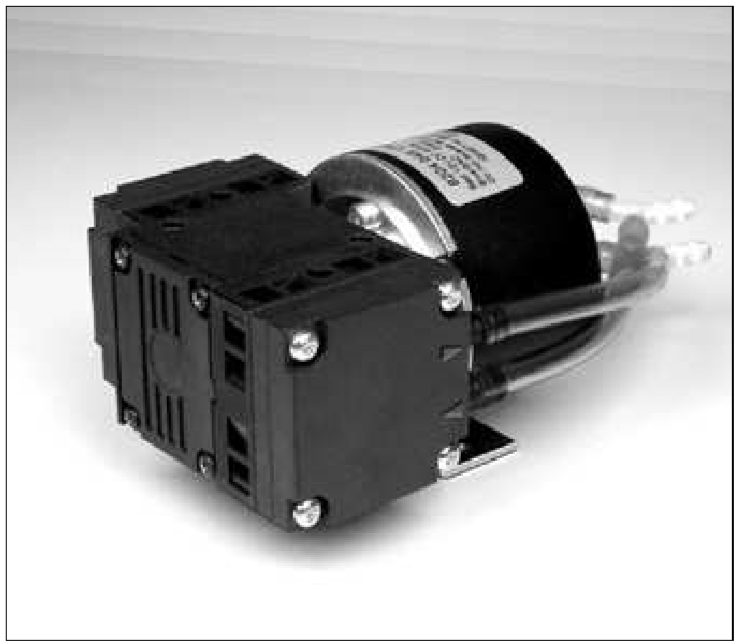
\includegraphics[width=6cm]{4-experiment-design/img/pump-850-1-2-kndc-b.png}
    \end{align*}
    \caption{KNF 850.1.2. KNDC B Miniature Diaphragm Pump}\label{fig:pumppic}
\end{figure}


\begin{figure}[H]
    \begin{align*}
        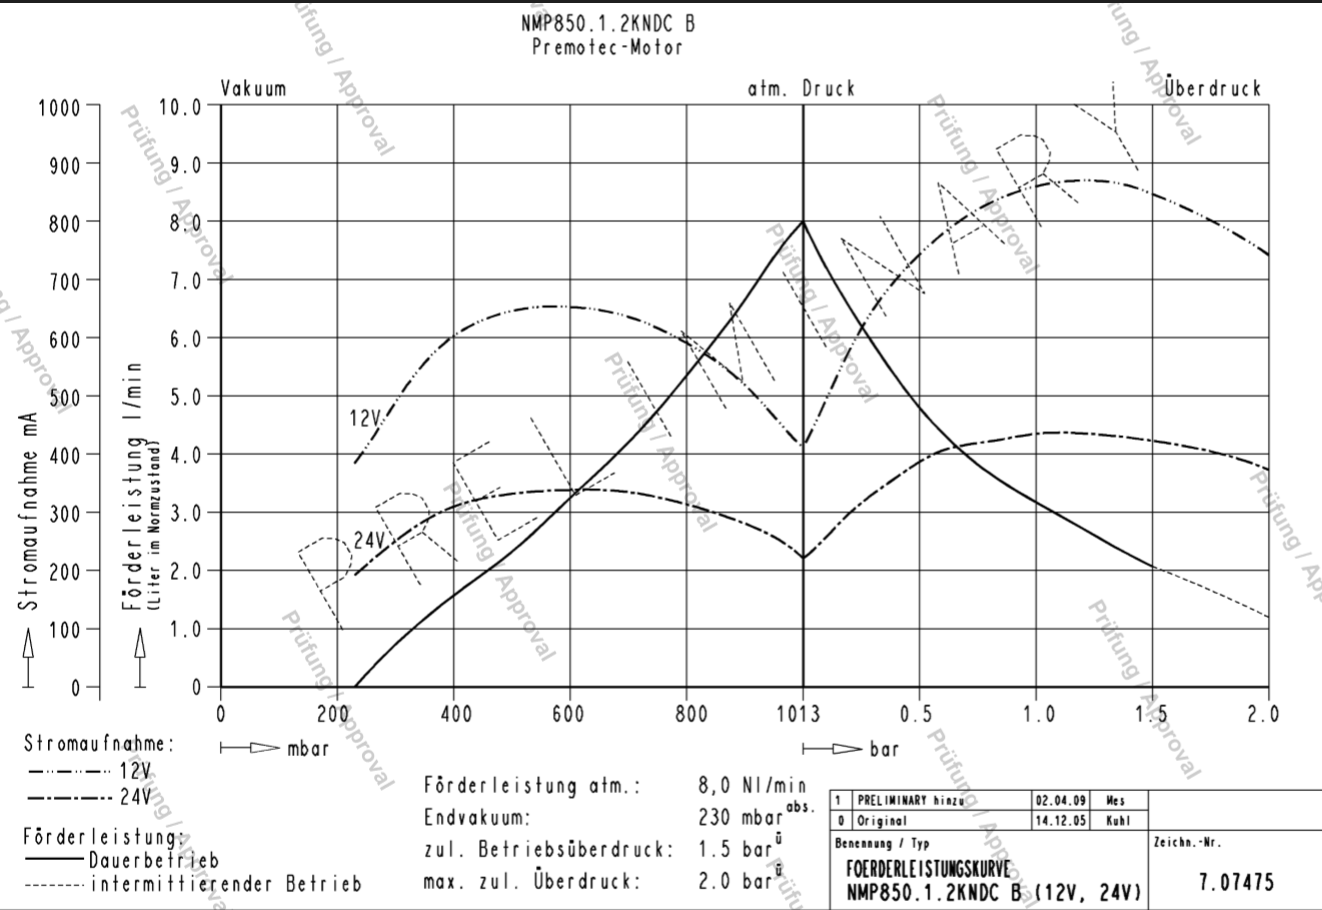
\includegraphics[width=15cm]{4-experiment-design/img/pump-flow-rate-current-graph.png}
    \end{align*}
    \caption{KNF 850.1.2. KNDC B Flow Rate and Current Draw to Pressure Graph.}\label{fig:pumpflowcur}
\end{figure}


\subsubsection{Electromagnetically Controlled Valves}
The filling of the sampling bags will be controlled by solenoid valves. For this purpose SMC solenoid valve VDW21-5G-1-01N-H-F-X23, Figure \ref{fig:valve}, has been selected. The valves will be normally closed through out the experiment with zero power consumption and will be open, when given power, to fill up the sampling bags at specific altitudes or to flush the tubes. In addition one valve will be on the AirCoil which will be opened shortly after take off and remain open the whole flight. This valve will be closed shortly before landing.

\begin{figure}[H]
    \begin{align*}
        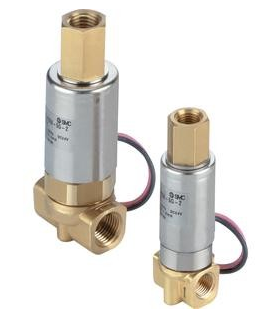
\includegraphics[width=6cm]{4-experiment-design/img/smc-valve.png}
    \end{align*}
    \caption{Valve}\label{fig:valve}
\end{figure}

The port size of the valve is 1/8" which is compatible with the gas analyzer. The coil can withstand temperature from -10 to 50 °C which is suitable for flight operations at high altitudes. Although the valve can operate under a maximum pressure drop of 0.2MPa it also needs to be tested at low pressure to check it operates as intended. 

\subsubsection{Switching Circuits}
The valves, pump and heaters will not take power from the Arduino but they still need to be controlled by it.In order to allow this control a connection will be made for each component to the Arduino with a switching circuit. This switching circuit will use a PhotoMOS, AQV251 \ref{fig:photoMOS}, to control which components are turned on at which time.

\begin{figure}[H]
    \begin{align*}
        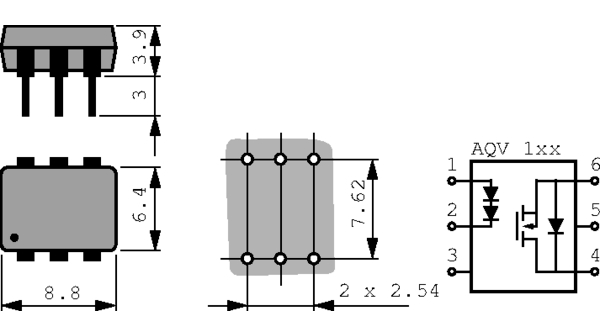
\includegraphics[width=6cm]{4-experiment-design/img/PhotoMOS.png}
    \end{align*}
    \caption{PhotoMOS AQV251}\label{fig:photoMOS}
\end{figure}


\raggedbottom